\documentclass[pdflatex,compress]{beamer}

%\usetheme[dark,framenumber,totalframenumber]{ElektroITK}
\usetheme[darktitle,framenumber,totalframenumber]{ElektroITK}
\usepackage{graphicx}
\usepackage{multicol}

\title{Data Communications}
\subtitle{Chapter 3 - Data Transmission}

\author{Mifta Nur Farid, M.T.}

\begin{document}

\maketitle

\begin{frame}
	\frametitle{Transmission Terminology}
	\begin{itemize}
		\item Data transmission occurs between transmitter and receiver over some transmission medium
		\item Communication is in the form of electromagnetic waves
		\item Guided media: Twisted pair, coaxial cable, optical fiber
		\item Unguided media (wireless): Propagation through air, vacuum, and seawater
	\end{itemize}
\end{frame}

\begin{frame}{Transmission Terminology}
	\begin{itemize}
		\item Direct link:
		\begin{itemize}
			\item No intermediate devices other than amplifiers or repeater used to increase signal strength.
		\end{itemize}
		\item Point-to-point: 
		\begin{itemize}
			\item Direct link between two devices
			\item Only 2 devices sharing medium
		\end{itemize}
		\item Multi-point
		\begin{itemize}
			\item More than two devices share the same medium
		\end{itemize}
	\end{itemize}
\end{frame}

\begin{frame}{Transmission Terminology}
	\begin{itemize}
		\item Simplex
		\begin{itemize}
			\item Signals are transmitted in only one direction
			\item One station is transmitter and the other is
			receiver
		\end{itemize}
		\item Half duplex 
		\begin{itemize}
			\item Both stations transmit, but only one at a time
		\end{itemize}
		\item Full duplex
		\begin{itemize}
			\item Both stations may transmit simultaneously
			\item The medium is carrying signals in both directions at the same time
		\end{itemize}
	\end{itemize}
\end{frame}

\begin{frame}
	\begin{center}
		\includegraphics[width=0.9\linewidth]{img/img01}
	\end{center}
\end{frame}

\begin{frame}
	\begin{center}
		\includegraphics[height=0.9\textheight]{img/img02}
	\end{center}
\end{frame}

\begin{frame}
	\frametitle{Sine Wave}
	\begin{itemize}
		\item The fundamental periodic signal
		\item Can be represented by three parameters
		\begin{itemize}
			\item Peak amplitude (A)
			\begin{itemize}
				\item Maximum value or strength of the signal over time
				\item Typically measured in volts
			\end{itemize}
			\item Frequency (f)
			\begin{itemize}
				\item Rate at which the signal repeats
				\item Hertz (Hz) or cycles per second
				\item Period (T) is the amount of time for one repetition
				\item T = 1/f
			\end{itemize}
			\item Phase ($ \phi $)
			\begin{itemize}
				\item Relative position in time within a single period of signal
			\end{itemize}
		\end{itemize}
	\end{itemize}
\end{frame}

\begin{frame}
	\begin{center}
		\includegraphics[height=0.9\textheight]{img/img03}
	\end{center}
\end{frame}

\begin{frame}
	\frametitle{Wavelength ($ \lambda $)}
	\begin{itemize}
		\item The wavelength of a signal is the distance occupied by a single cycle
		\item Can also be stated as the distance between two points of corresponding phase of two consecutive cycles
		\item Assuming signal velocity $ v $, then the wavelength is related to the period as $ \lambda = vT $
		\item Especially when $ v=c $\\
		$ c = 3\times10^8 $ m/s (speed of light in free space)
		\item Or equivalently $ \lambda f = v $
	\end{itemize}
\end{frame}

\begin{frame}
	\frametitle{Frequency Domain Concepts}
	\begin{itemize}
		\item Signals are made up of many frequencies
		\item Components are sine waves
		\item Fourier analysis can show that any signal is made up of components at various frequencies, in which each component is a sinusoid
		\item Can plot frequency domain functions
	\end{itemize}
\end{frame}

\begin{frame}
	\begin{center}
		\includegraphics[height=0.9\textheight]{img/img04}
	\end{center}
\end{frame}

\begin{frame}
	\begin{center}
		\includegraphics[height=0.9\textheight]{img/img05}
	\end{center}
\end{frame}

\begin{frame}
	\frametitle{Spectrum and Bandwidth}
	\begin{itemize}
		\item Spectrum: Range of frequencies contained in signal
		\item Absolute bandwidth: Width of spectrum
		\item Effective bandwidth (or just bandwidth): Narrow band of frequencies containing most energy
		\item DC Component: Component of zero frequency
	\end{itemize}
\end{frame}

\begin{frame}
	\begin{center}
		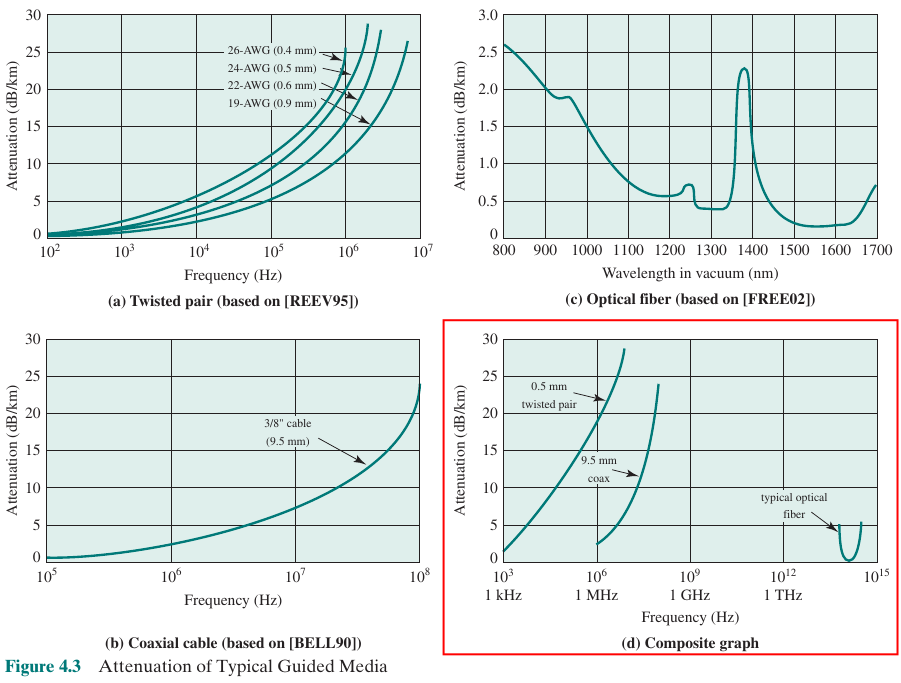
\includegraphics[height=0.9\textheight]{img/img06}
	\end{center}
\end{frame}

\begin{frame}
	\frametitle{Data Rate and Bandwidth}
	\begin{itemize}
		\item 	There is a direct relationship between data rate and bandwidth
		\item Any transmission system has a limited band of frequencies
		\item This limits the data rate that can be carried on the transmission medium
		\item Square waves have infinite components and hence an infinite bandwidth
		\item Most energy in first few components
		\item Limiting bandwidth creates distortions
	\end{itemize}
\end{frame}

\begin{frame}
	\begin{center}
		\includegraphics[height=0.8\textheight]{img/img07}
	\end{center}
\end{frame}

\begin{frame}
	\frametitle{Analog and Digital Data Transmission}
	\begin{itemize}
		\item Data: Entities that convey information
		\item Signal: Electric or electromagnetic representations of data
		\item Signaling: Physical propagation of the signal along a suitable medium
		\item Transmission: Communication of data by the propagation and processing of signals
	\end{itemize}
\end{frame}

\begin{frame}
	\begin{center}
		\includegraphics[height=0.8\textheight]{img/img08}
	\end{center}
\end{frame}

\begin{frame}
	\frametitle{Digital Data}
	\begin{itemize}
		\item Example:
		\begin{itemize}
			\item Text
			\item Character strings
			\item IRA
		\end{itemize}
	\end{itemize}
\end{frame}

\begin{frame}
	\begin{center}
		\includegraphics[width=\linewidth]{img/img09}
	\end{center}
\end{frame}

\begin{frame}
	\frametitle{Advantages and Disadvantages of\\Digital Signals}
	\begin{itemize}
		\item Generally cheaper
		\item Less susceptible to noise interference
		\item Suffer more from attenuation
	\end{itemize}
\end{frame}

\begin{frame}
	\begin{center}
		\includegraphics[width=0.9\linewidth]{img/img10}
	\end{center}
\end{frame}

\begin{frame}
	\frametitle{Video Signals}
	\begin{itemize}
		\item To produce a video signal a TV camera is used
		\item USA standard is 483 lines per frame, at a rate of 30 complete frames per second
		\begin{itemize}
			\item Actual standard is 525 lines but about 42 are lost during vertical retrace
		\end{itemize}
		\item  Horizontal scanning frequency is 525 lines $ \times $ 30 scans = 15750 lines per second
		\item Max frequency if line alternates between black and white as rapidly as possible
	\end{itemize}
\end{frame}

\begin{frame}
	\begin{center}
		\includegraphics[width=\linewidth]{img/img11}
	\end{center}
\end{frame}

\begin{frame}
	\begin{center}
		\includegraphics[width=\linewidth]{img/img12}
	\end{center}
\end{frame}

\begin{frame}
	\begin{center}
		\includegraphics[width=\linewidth]{img/img13}
	\end{center}
\end{frame}

\begin{frame}
	\frametitle{Analog and Digital Transmission}
	\begin{center}
		\includegraphics[width=0.8\linewidth]{img/img14}
	\end{center}
\end{frame}

\begin{frame}
	\frametitle{Move to Digital}
	\begin{itemize}
		\item \textbf{Digital technology}\\
		LSI and VLSI technology has caused a continuing drop in the cost and size of digital circuitry
		\item \textbf{Data integrity}\\
		The use of repeaters has made it possible to transmit data longer distances over lower quality lines while maintaining the integrity of the data
		\item \textbf{Capacity utilization}\\
		It has become economical to build transmission links of very high bandwidth, including satellite channels and optical fiber, and a high degree of multiplexing is needed to utilize such capacity effectively
	\end{itemize}
\end{frame}

\begin{frame}{Move to Digital}
	\begin{itemize}
		\item \textbf{Security and privacy}\\
		Encryption techniques can be readily applied to digital data and to analog data that have been digitized
		\item \textbf{Integration}\\
		Economies of scale and convenience can be achieved by integrating voice, video, and digital data
	\end{itemize}
\end{frame}

\begin{frame}
	\frametitle{Asynchronous and Synchronous Transmission}
	\textbf{Asynchronous}
	\begin{itemize}
		\item Strategy is to avoid the timing problem by not sending long, uninterrupted streams of bits
		\item Data are transmitted one character at a time, where each character is 5 to 8 bits in length
		\item Timing or synchronization must only be maintained within each character
		\item The receiver has the opportunity to resynchronize at the beginning of each new character
	\end{itemize}
\end{frame}

\begin{frame}{Asynchronous and Synchronous Transmission}
	\textbf{Synchronous}
	\begin{itemize}
		\item A block of bits is transmitted in a steady stream without start and stop codes
		\item Block may be many bits in length
		\item To prevent timing drift between transmitter and receiver, their clocks must somehow be synchronized
		\begin{itemize}
			\item Provide a separate clock line between transmitter and receiver
			\item Embed the clocking information in the data signal
		\end{itemize}
		\item Frame
		\begin{itemize}
			\item Data plus preamble, postamble, and control information
		\end{itemize}
	\end{itemize}
\end{frame}
\end{document}
